\documentclass{standalone}
\renewcommand{\sfdefault}{phv}

 \renewcommand{\familydefault}{\sfdefault}
%\fontfamily{helvetica}
  %\selectfont

\usepackage{tikz}
\usetikzlibrary{decorations.pathreplacing,positioning, arrows.meta}

\begin{document}         
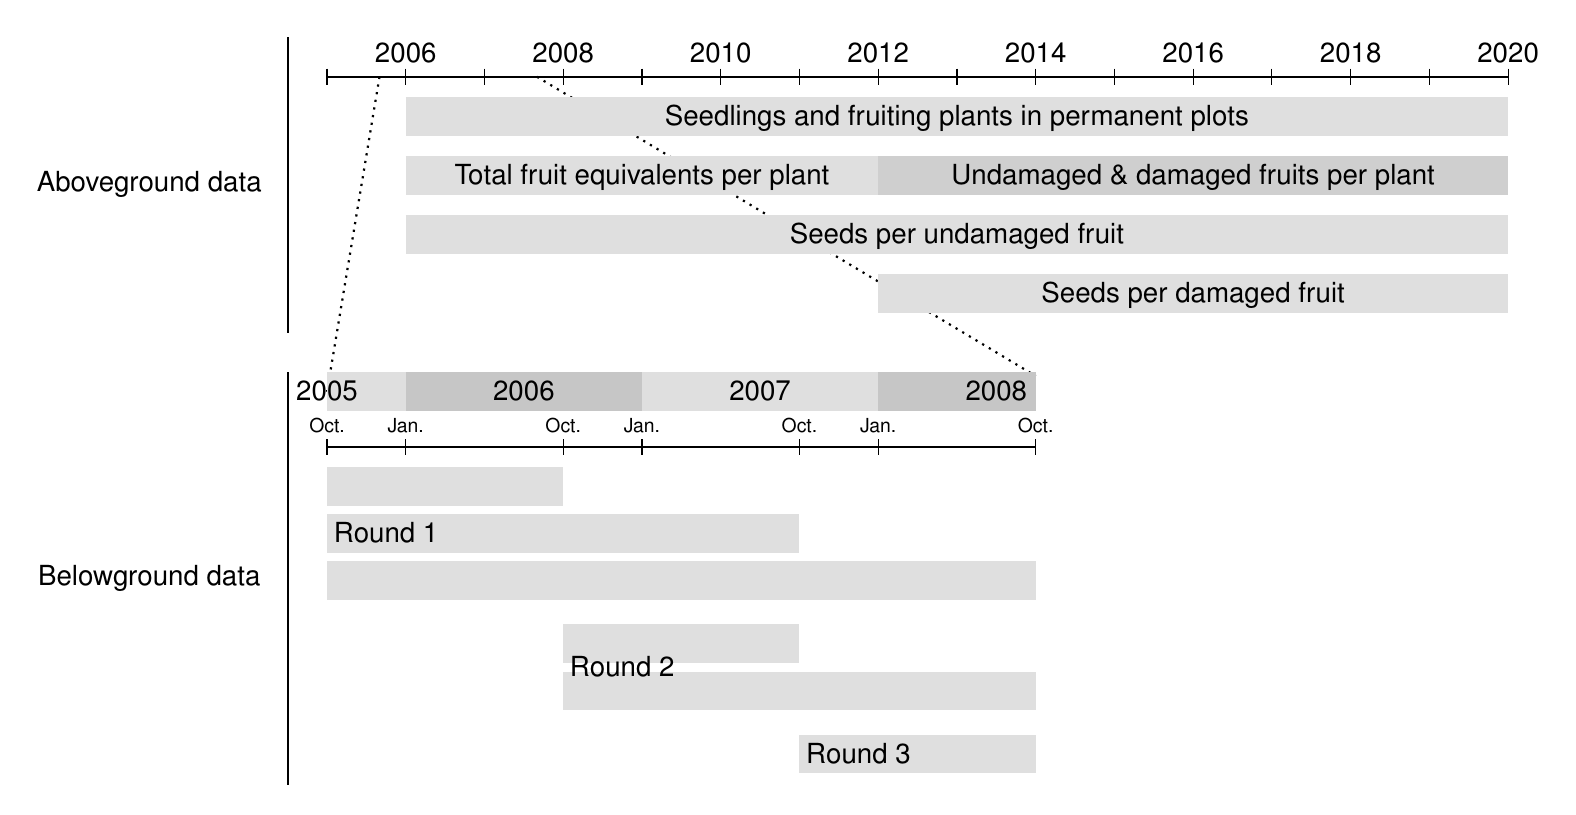
\begin{tikzpicture}

% draw horizontal line   
\draw[thick] (-1,0) -- (14,0) node[font=\scriptsize,below left=3pt and -8pt]{};

% draw vertical lines
\foreach \x in {-1,0,1,...,14}
\draw (\x cm,3pt) -- (\x cm,-3pt);

% dates
\foreach \x/\descr in {0/2006,2/2008,4/2010,6/2012,8/2014,10/2016,12/2018,14/2020}
\node[font=\normalsize, text height=1.75ex, text depth=.5ex] at (\x,.3) {\descr};

% dotted lines
\draw [draw, thick, dotted] (-{1/3},0) -- (-1,-4) ;
\draw [draw, thick, dotted] ({5/3},0) -- (8,-3.8) ;

% bars for permanent plots
\foreach \x/\perccol in
{0/50,1/50,2/50,3/50,4/50,5/50,6/50,7/50,8/50,9/50,10/50,11/50,12/50,13/50}
\draw[lightgray!\perccol!white, line width=14pt] 
(\x,-.5) -- +(1,0);

% bars for TFE
\foreach \x/\perccol in
{0/50,1/50,2/50,3/50,4/50,5/50}
\draw[lightgray!\perccol!white, line width=14pt] 
(\x,-1.25) -- +(1,0);

% bars for TFE
\foreach \x/\perccol in
{6/75,7/75,8/75,9/75,10/75,11/75,12/75,13/75}
\draw[lightgray!\perccol!white, line width=14pt] 
(\x,-1.25) -- +(1,0);

% bars for permanent plots
\foreach \x/\perccol in
{0/50,1/50,2/50,3/50,4/50,5/50,6/50,7/50,8/50,9/50,10/50,11/50,12/50,13/50}
\draw[lightgray!\perccol!white, line width=14pt] 
(\x,-2) -- +(1,0);

% bars for TFE
\foreach \x/\perccol in
{6/50,7/50,8/50,9/50,10/50,11/50,12/50,13/50}
\draw[lightgray!\perccol!white, line width=14pt] 
(\x,-2.75) -- +(1,0);

\node [font=\normalsize, text height=1.75ex, text depth=.5ex] at (7,-.5) {Seedlings and fruiting plants in permanent plots};
\node [font=\normalsize, text height=1.75ex, text depth=.5ex] at (3,-1.25) {Total fruit equivalents per plant};
\node [font=\normalsize, text height=1.75ex, text depth=.5ex] at (10,-1.25) {Undamaged \& damaged fruits per plant};
\node [font=\normalsize, text height=1.75ex, text depth=.5ex] at (7,-2) {Seeds per undamaged fruit};
\node [font=\normalsize, text height=1.75ex, text depth=.5ex] at (10,-2.75) {Seeds per damaged fruit};

% ADD SEED BAG DATA

% draw horizontal line   
\draw[thick] (-1,-4.7) -- (8,-4.7) node[font=\normalsize,below left=3pt and -8pt]{};

% draw vertical lines
\foreach \x in {-1,0,2,3,5,6,8}
\draw (\x cm,-4.6) -- (\x cm,-4.8);

% CALENDAR
\foreach \x/\perccol in
{-1/50,0/90,1/90,2/90,3/50,4/50,5/50,6/90,7/90}
\draw[lightgray!\perccol!white, line width=14pt] 
(\x,-4) -- +(1,0);

% dates
\foreach \x/\descr in {-1/2005,{1.5}/2006,{4.5}/2007,{7.5}/2008}
\node[font=\normalsize, text height=1.75ex, text depth=.5ex] at (\x,-4) {{\descr}};
\foreach \x/\descr in {-1/{Oct.},0/{Jan.},2/{Oct.},3/{Jan.},5/{Oct.},6/{Jan.},8/{Oct.}}
\node[font=\scriptsize, text height=1.75ex, text depth=.5ex] at (\x,-4.4) {{\descr}};


% ROUND 1
% Age 1
\foreach \x/\perccol in
{-1/50,0/50,1/50}
\draw[lightgray!\perccol!white, line width=14pt] 
(\x,-5.2) -- +(1,0);

% Age 2
\foreach \x/\perccol in
{-1/50,0/50,1/50,2/50,3/50,4/50}
\draw[lightgray!\perccol!white, line width=14pt] 
(\x,-5.8) -- +(1,0);

% Age 3
\foreach \x/\perccol in
{-1/50,0/50,1/50,2/50,3/50,4/50,5/50,6/50,7/50}
\draw[lightgray!\perccol!white, line width=14pt] 
(\x,-6.4) -- +(1,0);

% ROUND 2
% Age 1
\foreach \x/\perccol in
{2/50,3/50,4/50}
\draw[lightgray!\perccol!white, line width=14pt] 
(\x,-7.2) -- +(1,0);

% Age 2
\foreach \x/\perccol in
{2/50,3/50,4/50,5/50,6/50,7/50}
\draw[lightgray!\perccol!white, line width=14pt] 
(\x,-7.8) -- +(1,0);

% ROUND 3
% Age 1
\foreach \x/\perccol in
{5/50,6/50,7/50}
\draw[lightgray!\perccol!white, line width=14pt] 
(\x,-8.6) -- +(1,0);

\node [font=\normalsize, text height=1.75ex, text depth=.5ex] at (-.25,-5.8) {Round 1};
\node [font=\normalsize, text height=1.75ex, text depth=.5ex] at (2.75,-7.5) {Round 2};
\node [font=\normalsize, text height=1.75ex, text depth=.5ex] at (5.75,-8.6) {Round 3};

\draw [draw, thick] 
  (-1.5,.5) -- (-1.5,-3.25) node[midway,yshift=0em,xshift=-5em]{Aboveground data};
\draw [draw, thick]
  (-1.5,-3.75) -- (-1.5,-9) node[midway,yshift=0em,xshift=-5em]{Belowground data};  


\end{tikzpicture}

\end{document}
